\documentclass[conference]{IEEEtran}

\usepackage[utf8]{inputenc}
\usepackage[T1]{fontenc}
\usepackage[spanish,es-nodecimaldot]{babel}
\usepackage{microtype}
\usepackage{cite}
\usepackage{amsmath}
\usepackage{graphicx}
\usepackage{booktabs}
\usepackage{array}
\usepackage{tikz}
\usetikzlibrary{arrows.meta,positioning}
\usepackage{url}
\usepackage[hidelinks]{hyperref}

\addto\captionsspanish{\renewcommand{\tablename}{Tabla}}
\newcommand{\pc}{\,\%}
\hyphenation{pysenti-mento Unillanos CRISP-DM Streamlit}

\begin{document}

\title{Temas, sentimiento y emociones en comentarios de redes sociales de la Universidad de los Llanos: un an\'alisis exploratorio bajo CRISP-DM}

\author{
\IEEEauthorblockN{Juan Camilo Londo\~no Vel\'asquez}
\IEEEauthorblockA{Programa de Ingenier\'ia de Sistemas\\
Universidad de los Llanos\\
Villavicencio, Colombia\\
juan.londono.velasquez@unillanos.edu.co}
\and
\IEEEauthorblockN{Juan David Burgos Atuesta}
\IEEEauthorblockA{Programa de Ingenier\'ia de Sistemas\\
Universidad de los Llanos\\
Villavicencio, Colombia\\
jdburgos@unillanos.edu.co}
}

\maketitle

\begin{abstract}
Este trabajo presenta un an\'alisis exploratorio de 16.471 comentarios recopilados de publicaciones institucionales de Facebook, Instagram y YouTube de la Universidad de los Llanos. Se sigui\'o de forma integral la metodolog\'ia CRISP-DM para auditar y preparar los datos, estimar polaridad de sentimiento y emociones en espa\~nol con \texttt{pysentimiento}, estructurar una taxonom\'ia tem\'atica mediante reglas l\'exicas auditadas y desplegar los resultados agregados en una aplicaci\'on web interactiva en Streamlit. Tras excluir 586 registros sin texto, se analizaron 15.885 comentarios. La distribuci\'on afectiva estimada revel\'o un 58,2\pc{} neutral, 27,1\pc{} positivo y 14,6\pc{} negativo, predominando la clase emocional \emph{otros} (66,8\pc) y alegr\'ia (24,7\pc). La taxonom\'ia tem\'atica alcanz\'o una cobertura de temas espec\'ificos del 40,2\pc, aislando un 25,2\pc{} de mensajes sin contenido tem\'atico suficiente y reduciendo el residual sustantivo a 34,6\pc, destacando la identificaci\'on de la categor\'ia ``Protesta y movilizaci\'on'' (603 comentarios). En una muestra estratificada ($n = 198$), la validaci\'on humana independiente entre ambos autores arroj\'o un acuerdo inter-anotador de $\kappa = 0,515$ global y $\kappa = 0,623$ al excluir casos ambiguos. Frente al consenso humano acordado, las reglas coincidieron en la categor\'ia exacta en el 56,2\pc{} de los casos y detectaron la existencia de tema espec\'ifico en el 95,4\pc{} de las instancias pertinentes.
\end{abstract}

\begin{IEEEkeywords}
CRISP-DM, an\'alisis de sentimiento, emociones, redes sociales, comentarios, Streamlit, reglas l\'exicas, validaci\'on humana.
\end{IEEEkeywords}

%--------------------------------------------------------------------
\section{Introducci\'on}
Los comentarios emitidos en plataformas de redes sociales constituyen se\~nales relevantes sobre los asuntos que suscitan reconocimiento, dudas acad\'emicas, solicitudes administrativas y reacciones afectivas frente a una instituci\'on de educaci\'on superior. No obstante, el an\'alisis computacional de estos textos plantea desaf\'ios anal\'iticos sustantivos: la brevedad extrema de los mensajes, la dependencia del contexto de la publicaci\'on original, el uso intensivo de emojis y el l\'exico coloquial regional dificultan la clasificaci\'on autom\'atica confiable. Adem\'as, las estimaciones algor\'itmicas de sentimiento o tem\'atica no equivalen a opiniones verificadas ni representan por s\'i solas a la totalidad de la comunidad universitaria.

En este estudio, los dos autores desarrollamos un marco de procesamiento y an\'alisis descriptivo para organizar los comentarios recopilados de las cuentas oficiales de la Universidad de los Llanos (Unillanos) en tres dimensiones complementarias: \emph{polaridad} de sentimiento, \emph{emociones} b\'asicas estimadas y \emph{categor\'ias tem\'aticas} institucionales. El prop\'osito es proveer una herramienta descriptiva y transparente para auditar y explorar el conjunto capturado, explicitando sus l\'imites metodol\'ogicos. Las contribuciones principales comprenden:
\begin{itemize}
\item la consolidaci\'on y auditor\'ia de calidad de un corpus de 16.471 registros de tres plataformas, estandarizado a 15.885 unidades textuales analizables;
\item la implementaci\'on de un flujo de trabajo reproducible bajo el est\'andar CRISP-DM que articula modelos preentrenados de PLN en espa\~nol con reglas l\'exicas expl\'icitas con delimitadores de palabra;
\item la formulaci\'on y congelamiento criptogr\'afico de una taxonom\'ia tem\'atica institucional que incorpora categor\'ias cr\'iticas como protesta social y expresiones de aprecio;
\item una evaluaci\'on emp\'irica formal basada en anotaci\'on humana independiente de dos evaluadores ($n = 198$), midiendo acuerdo inter-anotador corregido por azar ($\kappa$) y desempe\~no por categor\'ia mediante intervalos de confianza de Wilson al 95\pc; y
\item el despliegue de una aplicaci\'on web interactiva en Streamlit que publica \'unicamente informaci\'on agregada con pol\'iticas de supresi\'on de grupos peque\~nos para salvaguardar la privacidad.
\end{itemize}

%--------------------------------------------------------------------
\section{Marco de referencia}
\textbf{CRISP-DM.} El modelo \emph{Cross-Industry Standard Process for Data Mining} (CRISP-DM) estructura el ciclo de vida de los proyectos de anal\'itica en seis fases iterativas: comprensi\'on del negocio, comprensi\'on de los datos, preparaci\'on, modelado, evaluaci\'on y despliegue \cite{chapman2000}. Su adopci\'on en este proyecto permiti\'o documentar y trazar rigurosamente las decisiones t\'ecnicas en cada etapa.

\textbf{Miner\'ia de opiniones y afecto en espa\~nol.} Para la estimaci\'on de polaridad y emociones se emple\'o la biblioteca especializada \texttt{pysentimiento} \cite{perez2021}, cuyos analizadores se fundamentan en RoBERTuito, un modelo de lenguaje basado en transformadores preentrenado exclusivamente con corpus masivos de redes sociales en espa\~nol \cite{perez2022}. El clasificador de emociones fue entrenado sobre el corpus EmoEvent \cite{plaza2020}, reconociendo las seis emociones b\'asicas de Ekman \cite{ekman1992} (\texttt{joy}, \texttt{anger}, \texttt{sadness}, \texttt{fear}, \texttt{surprise}, \texttt{disgust}) junto a una categor\'ia residual \texttt{others}.

\textbf{Validaci\'on de acuerdo inter-evaluador.} La concordancia entre anotadores independientes se evalu\'o mediante el coeficiente $\kappa$ de Cohen \cite{cohen1960}, el cual ajusta el acuerdo observado frente a la probabilidad de acuerdo atribuible al azar, interpret\'andose conforme a las escalas convencionales de Landis y Koch \cite{landis1977}. Los intervalos de precisi\'on y cobertura se estimaron con el m\'etodo asim\'etrico de Wilson \cite{wilson1927}.

%--------------------------------------------------------------------
\section{Datos y alcance}
La base unificada comprende \textbf{16.471 registros} brutos distribuidos en 12.089 de Facebook, 4.152 de Instagram y 230 de YouTube, asociados a 3.252 publicaciones institucionales. La auditor\'ia inicial confirm\'o la ausencia de identificadores duplicados. Tras retirar 586 registros que carec\'ian de texto, se consolid\'o un corpus analizable de \textbf{15.885 comentarios} (Tabla~\ref{tab:datos}). Del total analizado, 2.484 comentarios correspond\'ian a respuestas, las cuales se conservaron como unidades textuales independientes.

\begin{table}[!t]
\caption{Composici\'on del corpus analizable por plataforma}
\label{tab:datos}
\centering
\footnotesize
\begin{tabular}{lrrr}
\toprule
Plataforma & Filas brutas & Sin texto & Comentarios analizados \\
\midrule
Facebook  & 12.089 & 560 & 11.529 \\
Instagram & 4.152  & 26  & 4.126 \\
YouTube   & 230    & 0   & 230 \\
\midrule
Total     & 16.471 & 586 & 15.885 \\
\bottomrule
\end{tabular}
\end{table}

El estudio se delimit\'o a un alcance exploratorio y descriptivo sobre el material recolectado, absteni\'endose de establecer correlaciones temporales, inferencias causales o generalizaciones sobre la opini\'on no expresada en redes sociales.

%--------------------------------------------------------------------
\section{Metodolog\'ia bajo CRISP-DM}
El desarrollo del proyecto se ejecut\'o a trav\'es de las seis fases de CRISP-DM (Fig.~\ref{fig:crisp}).

\begin{figure*}[!t]
\centering
\begin{tikzpicture}[
  node distance=0.45cm,
  box/.style={draw, rounded corners=2pt, align=center, minimum width=2.55cm, minimum height=0.95cm, font=\footnotesize, inner sep=3pt},
  note/.style={align=center, font=\scriptsize, text width=2.55cm},
  arr/.style={-{Stealth[length=5pt]}, thick}]
\node[box] (a) {1. Comprensi\'on\\del negocio};
\node[box, right=of a] (b) {2. Comprensi\'on\\de los datos};
\node[box, right=of b] (c) {3. Preparaci\'on};
\node[box, right=of c] (d) {4. Modelado};
\node[box, right=of d] (e) {5. Evaluaci\'on};
\node[box, right=of e] (f) {6. Despliegue};
\foreach \x/\y in {a/b,b/c,c/d,d/e,e/f} \draw[arr] (\x) -- (\y);
\node[note, below=0.15cm of a] {objetivos descriptivos y preguntas clave};
\node[note, below=0.15cm of b] {auditor\'ia de calidad y distribuciones};
\node[note, below=0.15cm of c] {limpieza, muestras de 120 y 198};
\node[note, below=0.15cm of d] {\texttt{pysentimiento} + reglas l\'exicas};
\node[note, below=0.15cm of e] {validaci\'on humana independiente};
\node[note, below=0.15cm of f] {aplicaci\'on web en Streamlit};
\end{tikzpicture}
\caption{Flujo metodol\'ogico CRISP-DM ejecutado en el an\'alisis de comentarios institucionales.}
\label{fig:crisp}
\end{figure*}

\subsection{Comprensi\'on del negocio}
Se defini\'o el objetivo de estructurar los comentarios institucionales para facilitar una comprensi\'on auditada de las tem\'aticas y reacciones afectivas de la comunidad digital, orientada a la investigaci\'on acad\'emica y no a la evaluaci\'on de desempe\~no institucional.

\subsection{Comprensi\'on de los datos}
Se program\'o un m\'odulo de auditor\'ia que evalu\'o la distribuci\'on de frecuencias, completitud y caracteres especiales. Se identific\'o una disparidad marcada en el volumen: Facebook agrupa el 72,6\pc{} de los comentarios analizados, frente a 26,0\pc{} en Instagram y apenas 1,4\pc{} en YouTube. Asimismo, se cuantificaron 4.288 comentarios con s\'imbolos o emojis y 1.280 mensajes compuestos exclusivamente por emojis.

\subsection{Preparaci\'on de los datos}
Se excluyeron registros vac\'ios y se gener\'o una versi\'on normalizada del texto para an\'alisis de soporte l\'exico, preservando el texto original para los clasificadores neuronales. Mediante generaci\'on aleatoria con semilla determin\'istica fija (314159) se estratificaron dos subconjuntos representativos de 66 comentarios por plataforma: una muestra de 120 comentarios para evaluar polaridad y emoci\'on, y una muestra ampliada de 198 comentarios para la validaci\'on de la taxonom\'ia tem\'atica.

\subsection{Modelado}
El procesamiento afectivo se ejecut\'o mediante inferencia en CPU con RoBERTuito. La polaridad se clasific\'o en positiva (POS), neutral (NEU) o negativa (NEG). Para emoci\'on, la clase \texttt{others} se reporta como ``sin emoci\'on b\'asica identificable'' para evitar colisiones conceptuales con la neutralidad de sentimiento.

Para la asignaci\'on tem\'atica, se construy\'o un clasificador de reglas l\'exicas determin\'isticas. Se establecieron categor\'ias sustantivas evaluadas con orden de precedencia fija mediante expresiones regulares con delimitadores de frontera de palabra (\texttt{\textbackslash b}). Dicha precedencia se congel\'o formalmente mediante su hash criptogr\'afico SHA-256 (\texttt{a69292d7\allowbreak{}38828d2b\allowbreak{}bd1c8569\allowbreak{}b5dea235\allowbreak{}b404e7cd\allowbreak{}59708e81\allowbreak{}1868bf0f\allowbreak{}969f3266}) antes de contrastarla con las anotaciones humanas.

\subsection{Evaluaci\'on}
La evaluaci\'on const\'o de dos fases humanas independientes realizadas a ciegas por ambos autores: una valoraci\'on afectiva sobre 120 comentarios y una auditor\'ia tem\'atica sobre 198 comentarios, cuantificando coeficientes de acuerdo $\kappa$ y contrastando las etiquetas concordantes contra las reglas congeladas.

\subsection{Despliegue}
Se desarroll\'o una aplicaci\'on en Streamlit estructurada en vistas tem\'aticas y anal\'iticas. Para mitigar riesgos de privacidad, la aplicaci\'on opera exclusivamente sobre tablas precalculadas agregadas, aplicando supresi\'on en celdas con conteos inferiores a diez registros ($n < 10$).

%--------------------------------------------------------------------
\section{Resultados}

\subsection{Distribuci\'on global de sentimiento y emociones}
La Tabla~\ref{tab:sent-emo} resume los resultados afectivos en el corpus de 15.885 comentarios. Predomina el sentimiento neutral (58,2\pc), mientras que la categor\'ia \texttt{others} abarca dos de cada tres comentarios en emoci\'on (66,8\pc). La alegr\'ia representa la emoci\'on espec\'ifica predominante (24,7\pc), en tanto que las emociones aversivas registran baja frecuencia (enojo 5,0\pc, tristeza 2,9\pc, miedo 0,1\pc{} y disgusto $<$0,1\pc).

\begin{table}[!t]
\caption{Distribuci\'on de sentimiento y emoci\'on estimados ($N=15.885$)}
\label{tab:sent-emo}
\centering
\footnotesize
\begin{tabular}{@{}lrr@{\hspace{1.2em}}lrr@{}}
\toprule
\multicolumn{3}{c}{Polaridad de sentimiento} & \multicolumn{3}{c}{Emoci\'on predominante} \\
\cmidrule(r){1-3}\cmidrule(l){4-6}
Clase & $n$ & \% & Clase & $n$ & \% \\
\midrule
Neutral  & 9.250 & 58,2 & Otros (\texttt{others}) & 10.615 & 66,8 \\
Positivo & 4.312 & 27,1 & Alegr\'ia   & 3.916  & 24,7 \\
Negativo & 2.323 & 14,6 & Enojo      & 799    & 5,0 \\
         &       &      & Tristeza   & 466    & 2,9 \\
         &       &      & Sorpresa   & 79     & 0,5 \\
         &       &      & Miedo      & 9      & 0,1 \\
         &       &      & Disgusto   & 1      & $<$0,1 \\
\bottomrule
\end{tabular}
\end{table}

\begin{figure}[!t]
\centering
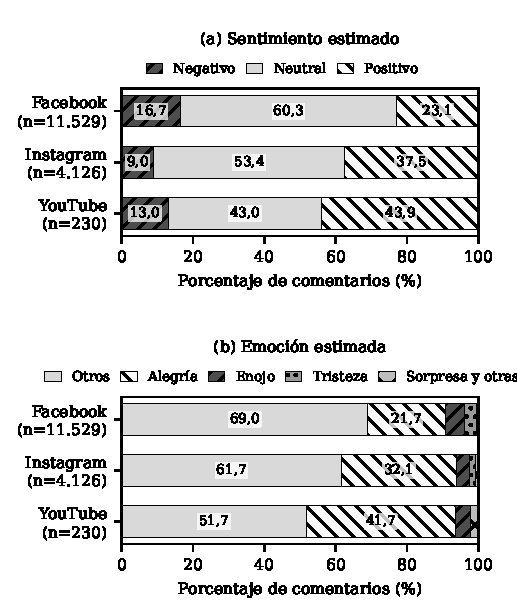
\includegraphics[width=\columnwidth]{fig_plataformas.pdf}
\caption{Distribuci\'on porcentual de sentimiento y emociones estimadas por plataforma en Unillanos.}
\label{fig:plat}
\end{figure}

La Fig.~\ref{fig:plat} evidencia diferencias descriptivas entre redes: Instagram exhibe una mayor proporci\'on de positividad (37,5\pc) y alegr\'ia (32,1\pc) en contraste con Facebook (23,1\pc{} y 21,7\pc). Por su parte, Facebook concentra la mayor proporci\'on de mensajes negativos (16,7\pc{} frente a 9,0\pc{} en Instagram).

\subsection{Distribuci\'on de la taxonom\'ia tem\'atica}
La Tabla~\ref{tab:temas_actualizados} expone la asignaci\'on tem\'atica obtenida tras implementar el esquema de reglas l\'exicas auditado. La cobertura de categor\'ias tem\'aticas espec\'ificas alcanz\'o el \textbf{40,2\pc} (6.380 comentarios), frente al 34,0\pc{} del diccionario inicial. Un 25,2\pc{} del corpus (4.004 comentarios) fue preclasificado como ``Sin contenido tem\'atico suficiente'', aislando comentarios reducidos a emojis, signos de puntuaci\'on o saludos breves. El residual sustantivo (``Otros temas no identificados'') se redujo de 66,0\pc{} a \textbf{34,6\pc} (5.501 comentarios).

\begin{table*}[t]
\centering
\footnotesize
\caption{Distribuci\'on tem\'atica final del corpus institucional y desglose por plataforma ($N = 15.885$).}
\label{tab:temas_actualizados}
\begin{tabular}{lrrrrrr}
\toprule
\textbf{Categor\'ia tem\'atica} & \textbf{$N$} & \textbf{\% Total} & \textbf{\% Facebook} & \textbf{\% Instagram} & \textbf{\% YouTube} & \textbf{\% Inicial} \\
\midrule
Protesta y movilizaci\'on & 603 & 3,8\% & 5,1\% & 0,2\% & 0,4\% & --- \\
Programas de acceso y bienestar & 421 & 2,7\% & 3,4\% & 0,7\% & 0,4\% & 2,9\% \\
Admisiones, inscripciones y matr\'iculas & 678 & 4,3\% & 5,0\% & 2,3\% & 3,0\% & 3,6\% \\
Informaci\'on, tr\'amites y certificados & 460 & 2,9\% & 3,1\% & 2,4\% & 3,5\% & 5,8\% \\
Oferta acad\'emica e investigaci\'on & 1.426 & 9,0\% & 9,1\% & 8,6\% & 12,6\% & 6,2\% \\
Infraestructura, sedes y tecnolog\'ia & 234 & 1,5\% & 1,5\% & 1,4\% & 2,2\% & --- \\
Eventos, cultura y actividades institucionales & 153 & 1,0\% & 0,8\% & 1,3\% & 2,2\% & 0,7\% \\
Felicitaciones y expresiones de aprecio & 2.405 & 15,1\% & 14,5\% & 16,3\% & 24,8\% & 14,8\% \\
\midrule
Sin contenido tem\'atico suficiente (social/emoji/menci\'on) & 4.004 & 25,2\% & 19,5\% & 41,4\% & 20,9\% & --- \\
Otros temas no identificados (residual sustantivo) & 5.501 & 34,6\% & 38,0\% & 25,5\% & 30,0\% & 66,0\% \\
\midrule
\textbf{Total corpus analizado} & \textbf{15.885} & \textbf{100,0\%} & \textbf{100,0\%} & \textbf{100,0\%} & \textbf{100,0\%} & \textbf{100,0\%} \\
\bottomrule
\end{tabular}
\end{table*}

\begin{figure}[!t]
\centering
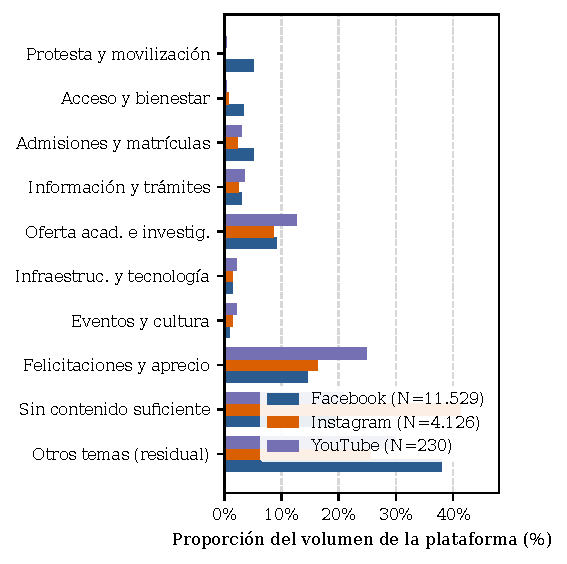
\includegraphics[width=\columnwidth]{fig_temas_plataforma.pdf}
\caption{Distribuci\'on porcentual de temas por plataforma de captura.}
\label{fig:temas_plat}
\end{figure}

Destaca la inclusi\'on en primer orden de precedencia de ``Protesta y movilizaci\'on'' (603 comentarios, 3,8\pc), que permiti\'o depurar 467 casos asociados a movilizaciones estudiantiles que anteriormente ca\'ian indebidamente en Oferta acad\'emica por la presencia de t\'erminos aislados. Asimismo, la Fig.~\ref{fig:temas_plat} refleja que Instagram concentra la mayor tasa de mensajes sin contenido tem\'atico (41,4\pc), mientras que las protestas se localizaron casi exclusivamente en Facebook (5,1\pc{} de su volumen).

\subsection{Cruce descriptivo de tema y sentimiento}
La Tabla~\ref{tab:tema_sentimiento_actualizado} presenta la distribuci\'on de polaridad en cada categor\'ia tem\'atica. Sobresale que ``Felicitaciones y expresiones de aprecio'' concentra un 82,5\pc{} de sentimiento positivo. Al respecto, es necesario enfatizar una \textbf{salvedad metodol\'ogica por construcci\'on}: esta categor\'ia se define mediante expresiones de elogio, cortes\'ia y reconocimiento, t\'erminos fuertemente correlacionados con la etiqueta positiva en los modelos de PLN; en consecuencia, dicha asociaci\'on no constituye un hallazgo emp\'irico independiente, sino un resultado inherente al dise\~no léxico de la regla.

\begin{table*}[!t]
\centering
\footnotesize
\caption{Distribuci\'on de polaridad de sentimiento estimada por \'area tem\'atica ($N = 15.885$). Se indica el porcentaje de celdas suprimidas por baja frecuencia ($n < 10$).}
\label{tab:tema_sentimiento_actualizado}
\begin{tabular}{@{}p{0.32\textwidth}rrrrr@{}}
\toprule
\textbf{Categor\'ia tem\'atica} & \textbf{$N$} & \textbf{\% NEG} & \textbf{\% NEU} & \textbf{\% POS} & \textbf{\% Supr.} \\
\midrule
Protesta y movilizaci\'on & 603 & 22,7\% & 75,1\% & 0,0\% & 2,2\% \\
Programas de acceso y bienestar & 421 & 13,5\% & 72,7\% & 4,3\% & 9,5\% \\
Admisiones, inscripciones y matr\'iculas & 678 & 25,8\% & 65,8\% & 1,8\% & 6,6\% \\
Informaci\'on, tr\'amites y certificados & 460 & 22,0\% & 66,1\% & 6,1\% & 5,9\% \\
Oferta acad\'emica e investigaci\'on & 1.426 & 25,9\% & 33,7\% & 38,6\% & 1,8\% \\
Infraestructura, sedes y tecnolog\'ia & 234 & 23,5\% & 44,9\% & 14,1\% & 17,5\% \\
Eventos, cultura y actividades & 153 & 0,0\% & 16,3\% & 61,4\% & 22,2\% \\
Felicitaciones y expresiones de aprecio & 2.405 & 1,3\% & 15,1\% & 82,5\% & 1,1\% \\
\midrule
Sin contenido tem\'atico suficiente & 4.004 & 2,5\% & 84,3\% & 12,8\% & 0,5\% \\
Otros temas no identificados & 5.501 & 21,6\% & 60,0\% & 18,4\% & 0,0\% \\
\midrule
\textbf{Total corpus} & \textbf{15.885} & \textbf{14,6\%} & \textbf{58,2\%} & \textbf{27,1\%} & \textbf{---} \\
\bottomrule
\end{tabular}
\end{table*}

\subsection{Validaci\'on humana de la taxonom\'ia tem\'atica}
Ambos autores evaluaron a ciegas una muestra estratificada de 198 comentarios (66 por plataforma). El acuerdo observado global fue del 60,6\pc{} (120/198), correspondiente a un $\kappa = 0,515$ (acuerdo moderado). Al excluir los comentarios se\~nalados con ambigüedad por los evaluadores ($n = 144$), el acuerdo ascendi\'o a \textbf{71,5\pc} con un $\kappa = \mathbf{0,623}$, se\~nalando una concordancia sustancial \cite{landis1977}. El an\'alisis revel\'o que el 27\pc{} de los comentarios presentaba ambigüedad sem\'antica inherente y el 47\pc{} depend\'ia estrictamente del contexto del post para desambiguarse.

Los 80 casos discordantes fueron resueltos mediante consenso humano deliberado. De las 198 filas, 4 persistieron como ambiguas consensuadas y fueron excluidas, consolidando 194 casos evaluables frente a las reglas congeladas (Tabla~\ref{tab:evaluacion_reglas_tematicas}). Para prevenir sobreinterpretaciones, se aplic\'o la regla de corte estricta $n < 10$ tanto sobre el soporte humano como sobre el total de predicciones del modelo.

\begin{table*}[!t]
\centering
\footnotesize
\caption{M\'etricas de validaci\'on de las reglas l\'exicas frente al consenso humano ($n = 194$). Intervalos de Wilson al 95\pc. Celdas con denominador menor a diez ($n < 10$) se declaran no interpretables.}
\label{tab:evaluacion_reglas_tematicas}
\begin{tabular}{@{}p{0.23\textwidth}p{0.10\textwidth}p{0.28\textwidth}p{0.28\textwidth}@{}}
\toprule
\textbf{Categor\'ia tem\'atica} & \textbf{Soporte} & \textbf{Precisi\'on (IC 95\%)} & \textbf{Recall (IC 95\%)} \\
\midrule
Protesta y movilizaci\'on & 12 & \textit{n < 10 (asig. 4)} & 33,3\% [13,8\%, 60,9\%] \\
Informaci\'on y tr\'amites & 19 & \textit{n < 10 (asig. 5)} & 21,1\% [8,5\%, 43,3\%] \\
Oferta acad\'emica & 13 & 38,1\% [20,8\%, 59,1\%] & 61,5\% [35,5\%, 82,3\%] \\
Felicitaciones y aprecio & 50 & 86,1\% [72,7\%, 93,4\%] & 74,0\% [60,5\%, 84,1\%] \\
\midrule
Otros temas (residual) & 14 & 20,3\% [12,0\%, 32,3\%] & 85,7\% [60,1\%, 96,0\%] \\
Sin contenido suficiente & 61 & 81,2\% [68,1\%, 89,8\%] & 63,9\% [51,4\%, 74,8\%] \\
\midrule
\multicolumn{4}{l}{\textit{Categor\'ias peque\~nas (Bienestar, Admisiones, Infraestructura, Eventos): n < 10}} \\
\bottomrule
\end{tabular}
\end{table*}

\begin{figure}[!t]
\centering
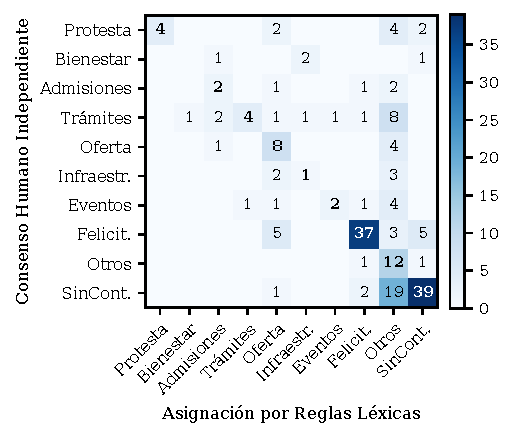
\includegraphics[width=\columnwidth]{fig_confusion_temas.pdf}
\caption{Matriz de confusi\'on entre el consenso humano y las reglas l\'exicas congeladas ($n = 194$).}
\label{fig:conf_temas}
\end{figure}

La contrastaci\'on emp\'irica evidenci\'o tres patrones estructurales fundamentales:
\begin{enumerate}
\item \textbf{Detecci\'on de tem\'atica sustantiva:} Cuando los evaluadores humanos identificaron la presencia de un tema espec\'ifico, las reglas determinaron que exist\'ia contenido no residual en el \textbf{95,4\pc} de los casos, omitiendo un 24,7\pc{} de casos sustantivos que fueron derivados al residual o a contenido m\'inimo.
\item \textbf{Coincidencia exacta de categor\'ia:} La coincidencia exacta entre la categor\'ia humana y la asignaci\'on l\'exica alcanz\'o el \textbf{56,2\pc} (109 aciertos de 194 casos evaluados, visible en la diagonal de la Fig.~\ref{fig:conf_temas}).
\item \textbf{Heterogeneidad del residual:} La categor\'ia ``Otros temas no identificados'' no es conceptualmente homog\'enea: en la muestra de revisi\'on, casi la mitad de los comentarios que las reglas enviaron al residual correspond\'ian a temas sustantivos espec\'ificos que escaparon a las palabras clave predefinidas.
\end{enumerate}

%--------------------------------------------------------------------
\section{Discusi\'on}
\textbf{Desempe\~no y l\'imites del enfoque l\'exico.} La obtenci\'on de un 56,2\pc{} de precisi\'on global frente al consenso humano demuestra que un sistema de reglas l\'exicas determin\'isticas con delimitadores de frontera (\texttt{\textbackslash b}) constituye una l\'inea base transparente y auditable para el an\'alisis institucional. No obstante, el 43,8\pc{} de discordancia subraya la fragilidad del filtrado exclusivamente superficial: t\'erminos gen\'ericos en Oferta acad\'emica (responsables del 48,2\pc{} de sus asignaciones) y expresiones de cortes\'ia en Felicitaciones (47,3\pc{} de asignaci\'on) generan solapamientos que solo un clasificador consciente del contexto sint\'actico puede resolver cabalmente.

\textbf{Ambigüedad y p\'erdida de contexto.} El hallazgo de que el 47\pc{} de los comentarios evaluados requiera el contexto de la publicaci\'on madre ratifica una restricci\'on inherente al procesamiento de redes sociales. Mensajes breves como ``\emph{\'Exitos}'' o solicitudes horarias carecen de carga sem\'antica aut\'onoma, explicando por qu\'e el acuerdo humano se eleva significativamente de $\kappa = 0,515$ a $\kappa = 0,623$ al descartar instancias ambiguas.

\textbf{Composici\'on del residual.} Que un 34,6\pc{} del corpus permanezca en la categor\'ia residual no debe interpretarse como una falla metodol\'ogica, sino como una representaci\'on honesta de la diversidad discursiva universitaria: preguntas at\'ipicas, quejas gremiales y debates pol\'iticos que desbordan cualquier cat\'alogo taxon\'omico cerrado.

%--------------------------------------------------------------------
\section{Limitaciones y consideraciones \'eticas}
\begin{enumerate}
\item \textbf{Representatividad muestral:} Las inferencias humanas provienen de una muestra estratificada de 198 casos dise\~nada para equilibrar plataformas, mas no para reflejar la proporci\'on poblacional exacta de Facebook.
\item \textbf{Regla de corte muestral:} En categor\'ias con soporte o asignaci\'on $n < 10$, las estimaciones de precisi\'on puntual y ponderada carecen de estabilidad matem\'atica y no deben generalizarse.
\item \textbf{Desbalance y ausencia de denominadores:} Los conteos absolutos reflejan la actividad de captura y no tasas normalizadas de interacci\'on por visualizaci\'on.
\item \textbf{Privacidad y \'etica:} Los datos crudos contienen identificadores de usuario y contenidos personales protegidos. Por ello, el despliegue p\'ublico se restringe estrictamente a informaci\'on agregada con protecci\'on de celdas peque\~nas ($n < 10$).
\end{enumerate}

%--------------------------------------------------------------------
\section{Conclusiones y trabajo futuro}
Se complet\'o un ciclo metodol\'ogico riguroso bajo el est\'andar CRISP-DM para auditar, modelar y evaluar 15.885 comentarios de la Universidad de los Llanos. La combinaci\'on de modelos RoBERTuito con reglas l\'exicas congeladas criptogr\'aficamente permiti\'o categorizar el 40,2\pc{} del corpus en \'areas institucionales espec\'ificas, aislar el 25,2\pc{} de mensajes sin contenido y caracterizar la protesta estudiantil (603 comentarios). La validaci\'on humana independiente evidenci\'o un acuerdo sustancial ($\kappa = 0,623$) y una concordancia del 56,2\pc{} con las reglas.

Como trabajo futuro se propone: (i) entrenar clasificadores supervisados mediante ajuste fino (\emph{fine-tuning}) de modelos de lenguaje preentrenados a partir de muestras anotadas; (ii) incorporar t\'ecnicas de modelado tem\'atico neural basadas en incrustaciones contextuales (BERTopic) para estructurar el residual sustantivo; (iii) evaluar la concatenaci\'on del texto de la publicaci\'on para resolver la dependencia contextual; y (iv) extender el an\'alisis hacia la din\'amica temporal de las publicaciones institucionales.

%--------------------------------------------------------------------
\section*{Disponibilidad y reproducibilidad}
Los resultados agregados se encuentran interactivos en \url{https://comentarios-unillanos.streamlit.app}. El c\'odigo fuente reproducible, scripts de auditor\'ia y documentaci\'on t\'ecnica de cada fase CRISP-DM est\'an disponibles en el repositorio p\'ublico \url{https://github.com/CamiloLVZ/analisis_de_comentarios_unillanos}.

\begin{thebibliography}{00}
\bibitem{chapman2000} P. Chapman \emph{et al.}, ``CRISP-DM 1.0: Step-by-step data mining guide,'' SPSS Inc., 2000.
\bibitem{perez2021} J. M. P\'erez \emph{et al.}, ``pysentimiento: A Python toolkit for sentiment analysis and SocialNLP tasks,'' arXiv:2106.09462, 2021.
\bibitem{perez2022} J. M. P\'erez, D. A. Furman, L. A. Alemany, and F. Luque, ``RoBERTuito: a pre-trained language model for social media text in Spanish,'' in \emph{Proc. 13th Language Resources and Evaluation Conf. (LREC)}, 2022, pp. 7235--7243.
\bibitem{plaza2020} F. M. Plaza-del-Arco, C. Strapparava, L. A. Ure\~na-L\'opez, and M. T. Mart\'in-Valdivia, ``EmoEvent: A multilingual emotion corpus based on different events,'' in \emph{Proc. 12th Language Resources and Evaluation Conf. (LREC)}, 2020, pp. 1492--1498.
\bibitem{ekman1992} P. Ekman, ``An argument for basic emotions,'' \emph{Cognition and Emotion}, vol. 6, no. 3--4, pp. 169--200, 1992.
\bibitem{cohen1960} J. Cohen, ``A coefficient of agreement for nominal scales,'' \emph{Educational and Psychological Measurement}, vol. 20, no. 1, pp. 37--46, 1960.
\bibitem{landis1977} J. R. Landis and G. G. Koch, ``The measurement of observer agreement for categorical data,'' \emph{Biometrics}, vol. 33, no. 1, pp. 159--174, 1977.
\bibitem{wilson1927} E. B. Wilson, ``Probable inference, the law of population, and the frequency of error,'' \emph{Journal of the American Statistical Association}, vol. 22, no. 158, pp. 209--212, 1927.
\end{thebibliography}

\end{document}
